\section*{Pub Crawl}
To investigate correlations in the OSM dataset, we provide a combined visualization
called \emph{Pub Crawl}
which shows the average minimum inter-pub distance and the average
minimum pub to ATM distance within each administrative area.
The two dimensions are mapped to hue
and saturation respectively, allowing to visualize them as
choropleth map (\figref{crawl}).
The two measures do not seem to be strongly correlated, but the visualization might
be helpful for anyone planning to go bar-hopping in Berlin.
\begin{figure}[b]
\centering
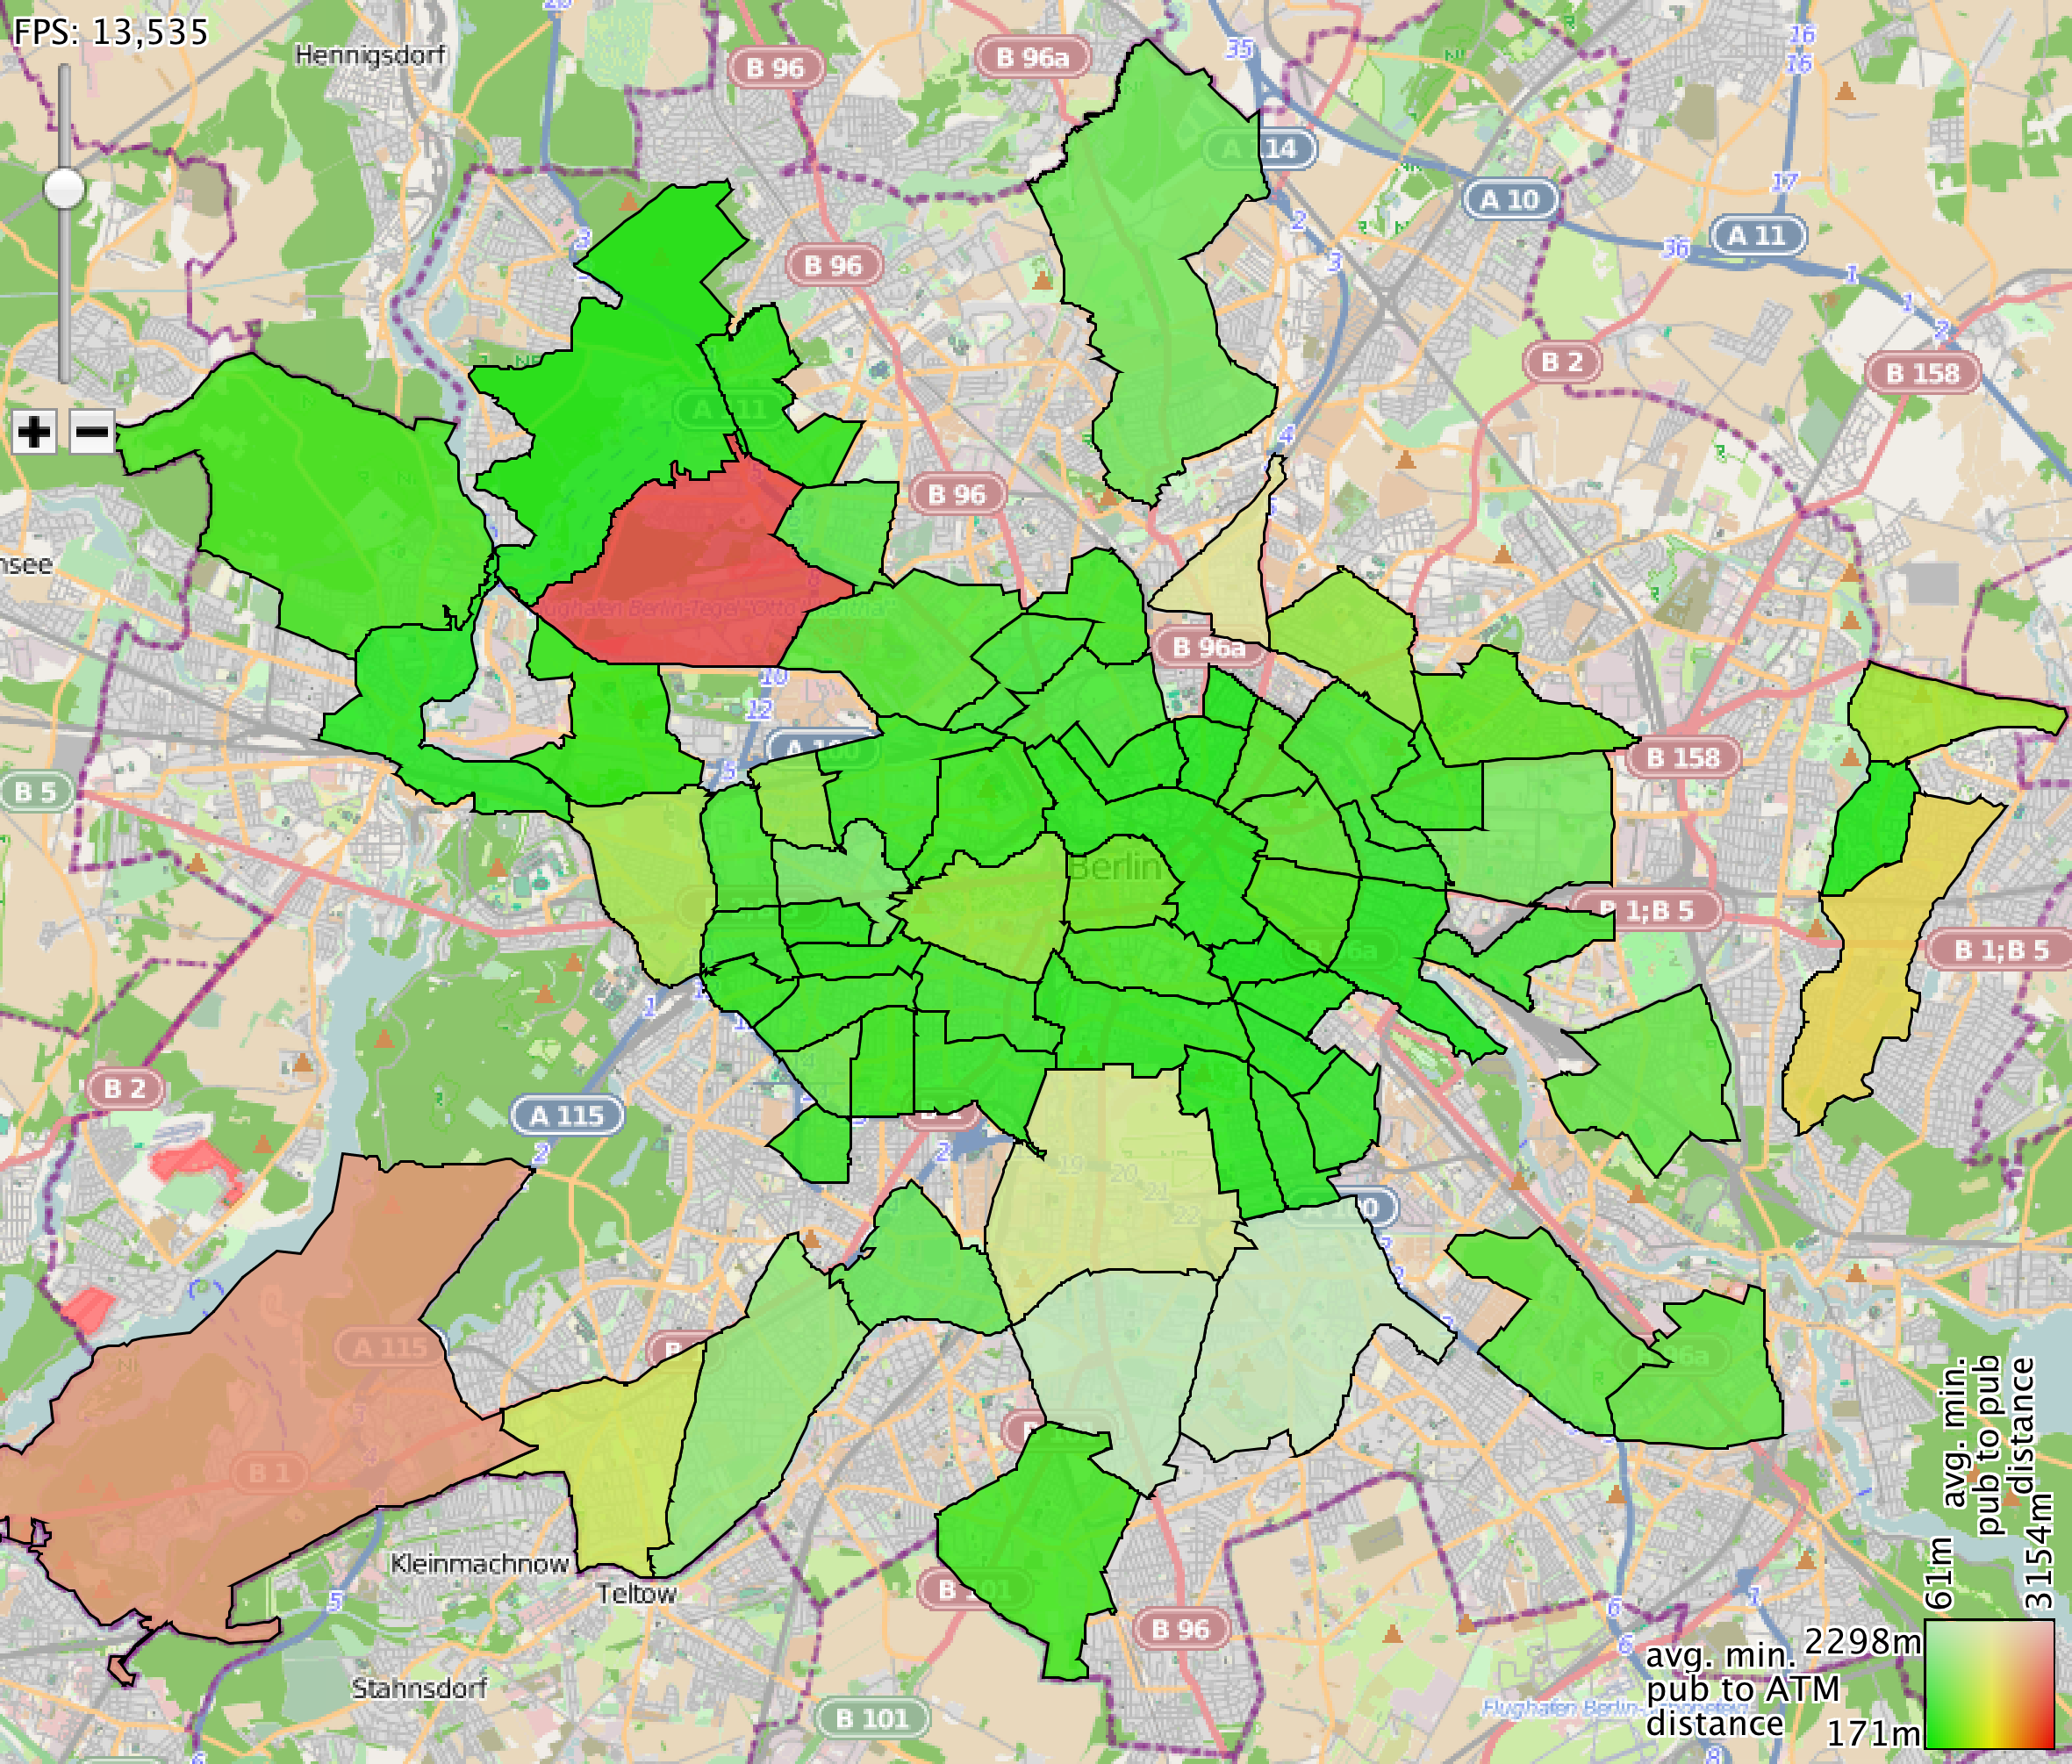
\includegraphics[width=0.6\linewidth]{imgs/crawl}
\caption{\emph{Pub Crawl} showing inter-pub distances 
and the average minimum pub to ATM distance.}
\label{fig:crawl}
\end{figure}
\section*{Open Wi-Fi}
As additional dataset we use data of open Wi-Fi hotspots in
the area of Berlin.
The data is displayed as a heatmap.

The dataset originally consisted only of plain-text street addresses
of public institutions, hotels, bars, restaurants, coffee places, and
other businesses with open Wi-Fi hotspots.
With the Google geocoding API we retrieved street addresses for all buildings
from the given dataset.
Next, we assigned Hotspots to buildings by matching addresses between the two datasets.

The heatmap is computed in a mesh of
arbitrary size. Each cell is computed by adding
the nearest distances of all buildings with a
hotspot together.
Since this is computationally expensive
we start with a loose mesh and refine it up to one pixel per cell while the
user is inactive.

Looking at the heatmap reveals some areas with higher density of open hotspots.
Namely the center of the city (Mitte), around the Sony Center,
in Prenzlauer Berg, and the area around Simon-Dach-Str.
and around Kürfürstendamm.
Those areas are known for being touristic and Mitte with Sony Center are additionally
areas with many businessmen.
As hotspots are likely to be in a restaurant, bar, or caf\'{e}
this seems to be due to the high demand for internet
from tourists (having no alternative) and businessmen (needing to
be online during lunch).
\begin{figure}
\centering
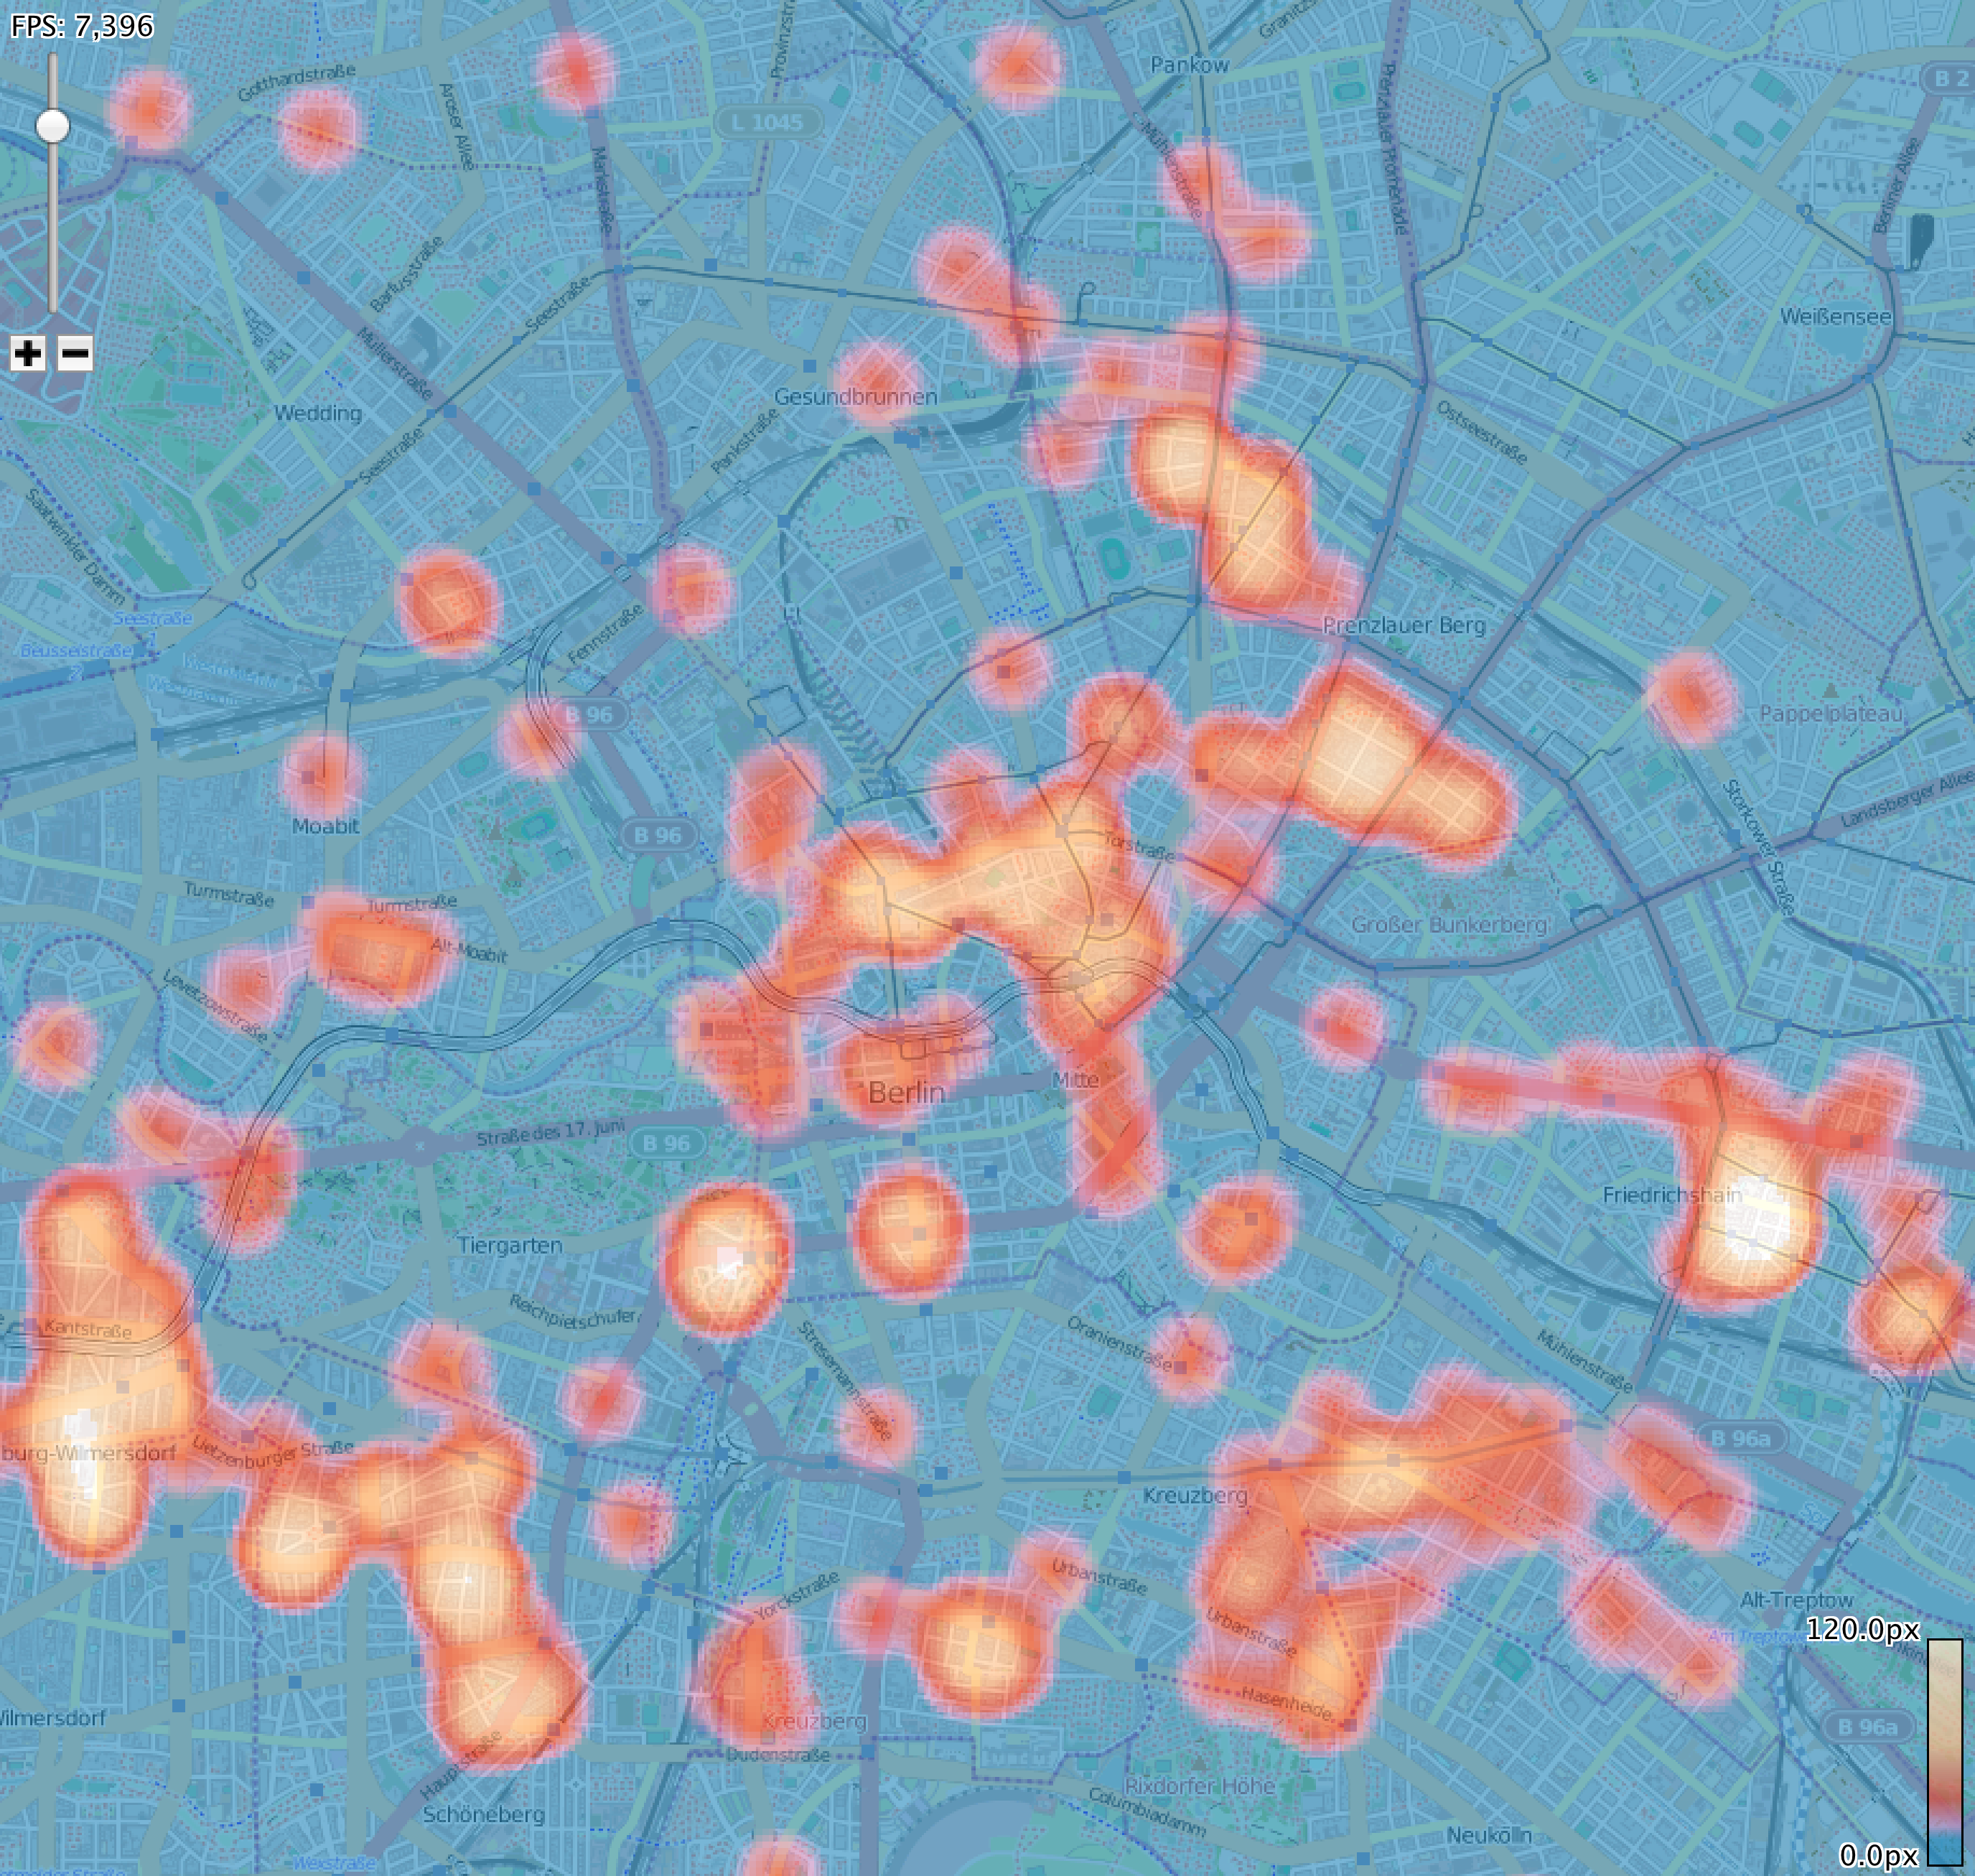
\includegraphics[width=0.45\linewidth]{imgs/heat}
\caption{The heatmap of free hotspots in Berlin.
The white spot to the right is the area around Simon-Dach-Str.}
\label{fig:heat}
\end{figure}
Based on our visualization of the hotspot data, we hypothesized that the hotspot locations
are unevenly distributed, with a greater density near the city center.
To investigate this further, we computed a distribution of the hotspots w.r.t. their
distance from the centroid of Berlin and compared it to the distribution that would
result from a uniform hotspot density all over Berlin. Both distributions are visualized
as step functions in \figref{wifi_distributions}. Although this simple approach does
not permit conclusions regarding the significance of the apparent differences,
it does support our hypothesis.
\begin{figure}[h]
	\centering
	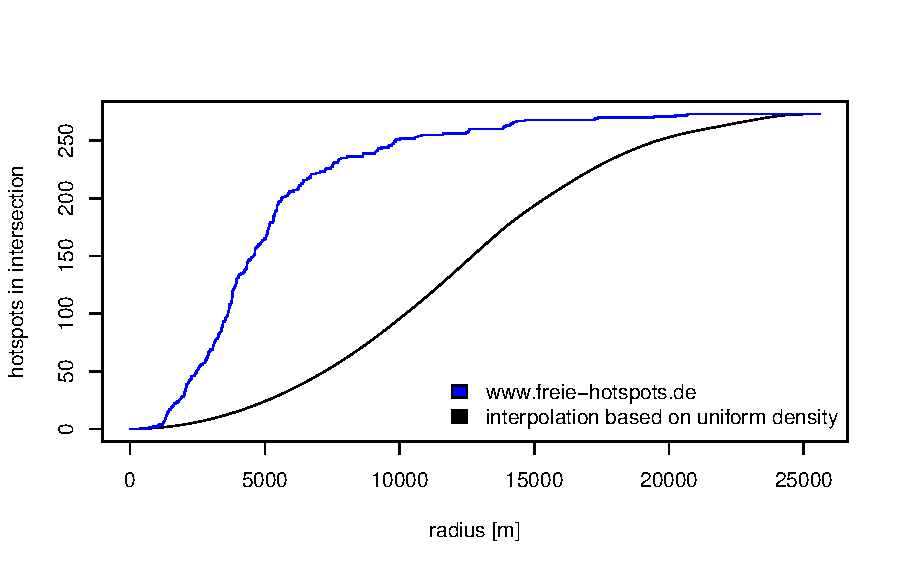
\includegraphics[scale=0.35]{imgs/wifi_distributions.pdf}
	\caption{Number of hotspots within the centroid of Berlin.}
	\label{fig:wifi_distributions}
\end{figure}
